\documentclass{article}
\usepackage{graphicx}
\usepackage{setspace}
\usepackage{hyperref}
\usepackage{fvextra}

\begin{document}

\bibliographystyle{plain}

\begin{titlepage}
    \centering
    
    % UCC Crest (clickable link)
    \vspace*{1.5cm}
    \href{https://www.ucc.ie/en/}{%
        
\includegraphics[width=0.25\textwidth]{img/ucc_crest.png}
    }
    
    \vspace{2cm}

    % Title
    {\Huge\bfseries Web-Based Tool for Observing\\[0.3cm]
    and Analysing Online Communities \par}
    
    \vspace{2.5cm}
    
    % Author
    {\Large Dylan De Faoite \par}
    
    \vspace{0.5cm}
    
    % Date
    {\large April 2026 \par}
    
    \vfill
    
    % Degree + Institution
    {\large
    Bachelor of Science in Computer Science \\[0.2cm]
    University College Cork \\[0.2cm]
    Supervisor: Paolo Palmeiri
    \par}
    
    \vspace{1.5cm}
    
\end{titlepage}

\tableofcontents
\newpage 

\section{Introduction}
This project presents the design and implementation of a web-based analytics engine for the exploration and analysis of online discussion data. Built using \textbf{Flask and Pandas}, and supplemented with \textbf{Natural Language Processing} (NLP) techniques, the system provides an API for extracting structural, temporal, linguistic, and emotional insights from social media posts. A React-based frontend delivers interactive visualizations and user controls, the backend architecture implements analytical pipeline for the data, including data parsing, manipulation and analysis.

\vspace{0.5cm}
Beyond its technical objectives, the system is conceptually informed by approaches from \textbf{digital ethnography} and computational social science. Traditional Ethnography is the practice of studying individual or group culture from the point of view of the subject of the study. Digital ethnography seeks to understand how social relations, topics and norms are constructed in online spaces.

\subsection{Motivation}
There are many beneficiaries of a digital ethnography analytic system: social scientists gain a deeper understanding of contemporary culture and online communities; businesses and marketers can better understand consumer behaviour and online engagement; educators and designers can improve digital learning environments and user experiences; and policymakers can make informed decisions regarding digital platforms, online safety, and community regulation.

\subsection{Goals \& Objectives}
\begin{itemize}
    \item \textbf{Collect data ethically}: enable users to link/upload text, and interaction data (messages etc) from specified online communities. Potentially an automated method for importing (using APIs or scraping techniques) could be included as well.
    \item \textbf{Organise content}: Store gathered material in a structured database with tagging for themes, dates, and sources.
    \item \textbf{Analyse patterns}: Use natural language processing (NLP) to detect frequent keywords, sentiment, and interaction networks.
    \item \textbf{Visualise insights}: Present findings as charts, timelines, and network diagrams to reveal how conversations and topics evolve.
\end{itemize}

\subsection{The Cork Dataset}

A defining feature of this project is its focus on a geographically grounded dataset centred on \textbf{Cork, Ireland}. The system analyses publicly available discussions relating to Cork drawn from multiple online platforms:

\begin{itemize}
    \item The \textbf{r/Cork} subreddit
    \item The \textbf{r/Ireland} subreddit using a Cork-specific search filter
    \item \textbf{YouTube} videos retrieved using Cork-related search queries
    \item The \textbf{Boards.ie Cork section}
\end{itemize}

\newpage
\section{Background}

\subsection{What is Digital Ethnography?}
Digital Ethnography is the study of cultures and interactions in various online spaces, such as forums, posts and video comments. The goal is not only to describe the high-level statistics such as number of posts and posts per day, but also analyse people's behaviour at an interactional and cultural level, delving into common phrases, interactions patterns and common topics and entities.

There are multiple methods to carry out digital ethnography, such as online participant observation through automated or manual methods, digital interviews via text or video or tracing digital footprints. 

Compared to traditional ethnography, digital ethnography is usually faster and more cost-effective due to the availability of large swathes of data across social media sites such as Reddit, YouTube, and Facebook and lack of need to travel. Traditional ethnography often relied on in-person interviews and in-person observation of communities

\subsubsection{Traditional Ethnography}
Ethnography originated in the late nineteenth and early twentieth centuries as a method for understanding cultures through long-term fieldwork. The goal was not just to describe behaviour, but to show how people made sense of that world. Over time, ethnography grew beyond anthropology into sociology, media studies, education, and human computer interaction, becoming a broadly used qualitative research approach. Traditional ethnography was closely tied to physical locations: villages, workplaces or towns. However, as communication technologies developed and social life increasingly took place through technological mediums, it was no longer tied to a physical place. Researchers questioned whether social interactions could still be studied properly if they were no longer tied to physical places.

\subsubsection{Transition to Digital Spaces}
The rise of the internet in the late twentieth century massively changed social interaction. Online forums, emails, SMS and social media platforms became central to human communication. All types of groups and identities were constructed. As a result, ethnographic methods were adapted to study these emerging digital environments. Early work in this area was referred to as "virtual ethnography" or "digital ethnography", where online spaces began to mixed and intertwine with traditional cultural spaces.

Digital ethnography gives us new challenges to overcome in comparison to traditional ethnography. The field is distributed across platforms, devices and online-offline interactions. For example, a digital ethnographer studying influencer culture might examine Instagram posts, comment sections, private messages, algorithms, and also conduct interviews or observe offline events. This transitions requires flexibility, since researchers can no longer rely solely on face-to-face interactions.

\subsection{Online Communities}
There are many different types of online communities, often structured in various ways, with many different types of users, norms and power dynamics. These communities can range from large-scale social networking platforms and discussion forums to niche interest. Each type of community fosters different forms of interaction, participation, and identity construction.

Participation within these communities is usually not evenly distributed. The majority of users are passive consumers (lurkers), a smaller percentage contribute occasionally, and a very small core group produces most of the content. This uneven contribution structure has significant implications for digital ethnography, as visible discourse may disproportionately reflect the perspectives of highly active members rather than the broader community. This is particularly evident in some reputation-based systems such as Reddit, which allows for the opinions of a few to rise above the rest.

Examples of digital spaces include:
\begin{itemize}
    \item \textbf{Social media platforms} (e.g., Facebook, Twitter, Instagram) where users create profiles, share content, and interact with others.
    \item \textbf{Online forums and communities} (e.g., Reddit, Boards.ie) where users engage in threaded discussions around specific topics or interests.
    \item \textbf{Video platforms} (e.g., YouTube) where users share and comment on video content, often fostering communities around specific channels or topics.
    \item \textbf{Messaging apps} (e.g., WhatsApp, Discord) where users engage in private or group conversations, often with a more informal and intimate tone.
\end{itemize}

\subsection{Digital Ethnography Metrics}
This section describes common keywords and metrics use to measure and quantify online communities using digital ethnography.

\subsubsection{Sentiment Analysis}
Sentiment Analysis involves capturing the emotions associated with a specific post, topic or entity. This type of analysis can be as simple as classifying a post as "positive" or "negative", or classifying a post into a set of pre-existing emotions such as anger, joy or sadness.

\subsubsection{Active vs Passive Participation}
Not everyone in an online community participates in the same way. Some users post regularly and leave comments while others might simply read content without ever contributing anything themselves. Some might only contribute occasionally.

This distinction between active and passive participation (passive users are often referred to as "lurkers") is important in digital ethnography, because looking only at posts and comments can give a misleading picture of how large or engaged a community actually is. 

\subsubsection{Temporal Activity Patterns}
Looking at when a community is active can reveal quite a lot about its nature and membership. A subreddit that peaks at 2am UTC might have a mostly American userbase, while one that is consistently active across all hours could suggest a more globally distributed community. Beyond timezones, temporal patterns can also capture things like how a community responds to external events, like a sudden spike in posting activity often corresponds to something newsworthy happening that is relevant to the community.

\subsubsection{Cultural Markers}
Cultural markers are the words, phrases, memes, and behaviours that are specific to a particular community and signal that someone is a member of it. These might include in-jokes, niche slang, recurring references, or even particular ways of formatting posts. In the context of digital ethnography, identifying these markers is useful because they reveal how communities build a shared identity and distinguish themselves from outsiders.

Some patterns, such as usage of words like "we, us, our, ourselves", where posts are referring to themselves as a community might have different sentiment to posts where words like "they, them, their, themselves" are used. These are known as "identity markers" and they can be used to identify how welcoming a community might be to outsiders.

\subsubsection{Stance Markers}
Stance Markers refer to the usage of different phrasing patterns which can reveal the speakers attitude towards topics. There are different kinds of these phrasings, such as hedge, certainty, deontic and permission patterns.

\textbf{Hedge Patterns} are usually phrases that contain words like "maybe, possibly, probably, i think, i feel" and generally mean that someone is unsure or suspicious about something.

\textbf{Certainty Patterns} contain phrases like "definitely, certainly, clearly, obviously" and as the name suggests, imply certainty or assuredness.

\textbf{Deontic Patterns} contains phrases that imply obligation, such as "must, should, need, have to". In the context of online communities, these patterns are often used to assert authority or to reinforce communal norms and "unwritten rules."

\textbf{Permission Patterns} refer to phrases where someone is asking permision, like "can, allowed, ok, permitted". These patterns could serve as an indicator of a user's status within an online community.

\subsection{Natural Language Processing}
\textbf{Natural Language Processing} is a branch of artificial intelligence that allows machines to interpret, analyse and generate human language. The aim of NLP models is not only to understand single words individually, but to be able to understand the context of those words in a broader paragraph or story.

NLP can carry out many different types of tasks, such as classifying sentences or paragraphs, generating text content, extracting answers from text or even speech recognition in audio. However, even with the advances in NLP models, many challenges and limitations remain. These include understanding ambiguity, cultural context, sarcasm, and humour.

\subsubsection{Why Natural Language Processing?}
Digital ethnography traditionally relied on manual reading of texts and interviews. These approaches are valuable for deep interpretive analysis, but they do not scale well to the volume of data generated in online communities. A single subreddit might contain hundreds of thousands of posts and comments, far beyond what any single researcher could read and analyse by hand.

NLP techniques can be used to automatically process and analyse large volumes and applying ethnographic methods at scale. For example, NLP can be used to identify common themes and topics in a subreddit, track how these themes evolve over time, and even detect the emotional tone of discussions. This allows researchers to gain insights into the dynamics of online communities that would be impossible to achieve through manual analysis alone.

\subsubsection{Sentiment Analysis}
\textbf{Sentiment Analysis} involves determining the emotional tone behind a piece of text. It is commonly used to classify text as positive, negative, or neutral. This technique is widely applied in areas such as customer feedback analysis, social media monitoring, and market research. More advanced sentiment analysis models can detect nuanced emotions, such as frustration, satisfaction, or sarcasm, although accurately identifying these emotions remains a challenge.

\subsubsection{Named Entity Recognition}
\textbf{Named Entity Recognition (NER)} is the process of identifying and classifying key entities within a text into predefined categories like names of people, organisations, locations, or dates. NER is essential for structuring unstructured text data and is often used in information extraction, search engines, and question-answering systems. Despite its usefulness, NER can struggle with ambiguous entities or context-dependent meanings.

\subsubsection{Topic Modelling}
\textbf{Topic Modelling} is a technique used in NLP to identify the main themes or topics present in a collection of text. Instead of analysing each sentence individually, topic modelling looks for patterns of words that frequently appear together, allowing it to group documents based on similar themes.

This method is often used to organise lots of unstructured data, such as news articles, research papers, or social media posts.

\subsubsection{Stop Words}
\textbf{Stop Words} are common words that are often filtered out in NLP tasks because they carry little meaningful information. Examples of stop words include "the", "is", "in", "and", etc. Removing stop words can help improve the performance of NLP models by reducing noise and focusing on more informative words. However, the choice of stop words can vary depending on the context and the specific task at hand.

For example, in a Cork-specific dataset, words like "ah", or "grand" might be considered stop words, as they are commonly used in everyday speech but do not carry significant meaning for analysis.

\subsection{Limits of Computation Analysis}
While computational methods enable large-scale observation and analysis of online communities, there are many limitations that must be acknowledged. Many limitations come from NLP techniques and the practical boundaries of computational resources.

Natural Language Processors will be central to many aspects of the virtual ethnography, such as emotional and topic classification. While these models are strong and have shown results in many areas, they are imperfect and may produce inaccurate or misleading results.

One key limitation is how the models will likely find it difficult to interpret context-dependent language. Online communities will often use sarcasm, irony or culturally specific references, all of which will be challenging to for NLP models to correctly interpret. For example, a sarcastic comment might be incorrectly classified as positive, despite conveying negativity.

In addition, the simplification of complex human interactions and emotions into discrete categories like "happy" or "sad" will more than likely overlook some nuance and ambiguity, even if the model is not inherently "wrong". As a result, the outputs of NLP models should be interpreted as indicative patterns rather than definitive representations of user meaning.

\subsubsection{Computational Constraints}
The performance and speed of the system will be influenced by the computational resources available during development and execution. While the system will attempt to use GPU acceleration during NLP inference, these resource may not always be available or may not be particularly strong should they exist.

\subsection{Cork Dataset}
The Cork dataset serves as the foundation for this project, providing a geographically and culturally grounded corpus for analysis. Rather than examining a globally distributed or topic-neutral community, the dataset centres on a single city with Cork, Ireland which allows the system's analytical outputs to be interpreted against a known social and cultural context.

The dataset is drawn from four distinct online platforms, each of which represents a structurally different mode of online community participation:

\begin{itemize}
    \item \textbf{r/Cork} — a dedicated subreddit for Cork residents and diaspora, characterised by threaded discussion, upvote-based content curation, and an established community identity with its own norms and recurring topics.
    \item \textbf{r/Ireland} (Cork-filtered) — the broader Irish national subreddit, filtered by Cork-related keywords, capturing how Cork is discussed within a wider national discourse rather than within its own community space.
    \item \textbf{YouTube} — video comments retrieved via Cork-related search queries, representing a flatter, less threaded interaction model and a potentially more casual or emotionally expressive register than forum-style platforms.
    \item \textbf{Boards.ie Cork section} — an older Irish forum platform with a distinct demographic profile and lower volume compared to Reddit, providing a counterpoint to the Reddit-dominant data and representing a longer-established form of Irish online community.
\end{itemize}

Reddit's hierarchical comment threading enables deep conversational analysis and reply-chain metrics, whereas YouTube comments are largely flat and unthreaded. Boards.ie occupies a middle ground, with linear threads but a more intimate community character. Taken together, the four sources offer variation in interaction structure, community age, demographic composition, and linguistic register, all of which are factors that the system's analytical modules are designed to detect and compare.

Due to data being collected across multiple platforms, they must be normalised into a single data model. Posts, comments, and metadata fields differ in schema and semantics across sources. A core design requirement of the system is the normalisation of these inputs into a unified event-based internal representation, allowing the same analytical pipeline to operate uniformly regardless of the source.

\newpage
\section{Analysis}

\subsection{Goals \& Objectives}
The objective of this project is to provide a tool that can assist social scientists, digital ethnographers, and researchers to observing and interpret online communities and the interactions between them. Rather than replacing the study of digital ethnography or the related fields, this tool aims to aid researchers analyse communities.

Specifically, the system aims to: 

\begin{itemize}
    \item \textbf{Enable scalable observation}: Provide researchers with the ability to process and explore large volumes of online discussion data that would be impractical to analyse manually.

    \item \textbf{Support mixed-method research}: Bridge quantitative computational analysis and qualitative ethnographic interpretation by presenting statistically derived insights that can inform deeper contextual study.

    \item \textbf{Reveal structural dynamics}: Expose interaction patterns such as reply networks, participation inequality, conversation depth, and influential contributors within a community.

    \item \textbf{Identify thematic structures}: Detect dominant topics, recurring phrases, and emerging themes using Natural Language Processing techniques.

    \item \textbf{Track emotional and cultural signals}: Analyse sentiment and emotion distributions across posts, users, and topics to better understand the affective tone of discussions and how it evolves over time.

    \item \textbf{Examine temporal evolution}: Provide time-series analysis of activity levels, topic trends, and emotional shifts, enabling longitudinal observation of community development.

    \item \textbf{Promote ethical data practices}: Restrict analysis to publicly available data, provide opt-out mechanisms for computationally intensive processing, and ensure responsible handling of user-generated content.
\end{itemize}

Ultimately, the project seeks to demonstrate how computational systems can aid and augment social scientists and digital ethnographers toolkits.

\subsection{Feasibility Analysis}
\subsubsection{NLP Limitations}
Online communities often use sarcasm, irony or context-specific references, all of which will be challenging for NLP models, especially weaker ones, to correctly interpret. In a Cork-specific dataset, this will be especially apparent due to the use of regional slang or informal grammar. 

Therefore, the outputs of the model for any single event should not be considered as definitive, but rather as an indicative pattern that is more likely to be correct when aggregated across the entire dataset. For example, while a single comment about a specific topic might be misclassified as positive, the overall sentiment of that topic across thousands of comments is more likely to reflect the true emotional tone of the community.

To account for NLP limitations, the system will:
\begin{itemize}
    \item Rely on \textbf{aggregated results} rather than individual classifications.
    \item Provide \textbf{context for outputs}, such as confidence scores where available.
    \item Allow \textbf{access to original text} behind each NLP result.
\end{itemize}

Overall, while NLP provides powerful tools for analysing large datasets, its limitations must be acknowledged and mitigated through careful design and interpretation of results.

\subsubsection{Data Normalisation}
Different social media platforms will produce data in many different formats. For example, Reddit data will have a much different reply structure to a forum-based platform like Boards.ie where there are no nested replies. Therefore, a core design requirement of the system is to normalise all incoming data into a single unified internal data model. This allows the same analytical functions to be applied across all data sources, regardless of their original structure.

Posts and comments are two different types of user-generated content, however when it comes to ethnographic analysis, they are both just "events" or information that is being shared by a user. From an ethnographic perspective, the distinction between a post and a comment is not particularly important, since they both represent user-generated content that contributes to the community discourse. Therefore, the system will normalise all posts and comments into a single "event" data model, which will allow the same analytical functions to be applied uniformly across all content. This also simplifies the data model and reduces the complexity of the analytical pipeline, since there is no need to maintain separate processing paths for posts and comments.

Though separate processing paths are not needed, the system will still retain metadata that indicates whether an event was originally a post or a comment, as well as any relevant structural information (e.g., parent-child relationships in Reddit threads).

\subsubsection{Scalability Constraints}
This system should be scalable enough to handle large datasets, but there are practical limits to how much data can be processed within reasonable timeframes, especially given the computational demands of NLP models.

Some of the data can be precomputed during the data ingestion phases, such as datetime column derivations and NLP outputs, which can speed up and make queries more efficient. However, the initial processing time of large datasets will still be significant, especially if the dataset contains hundreds of thousands of posts and comments.

To mitigate this, the system will:
\begin{itemize}
    \item Utilise GPU acceleration where available for NLP inference.
    \item Pre-compute some analytical results during data ingestion to speed up subsequent queries.
    \item Store NLP outputs in the database to avoid redundant processing.
    \item Implement asynchronous processing for long-running tasks.
\end{itemize}

Overall, while the system is designed to be scalable, it is important to set realistic expectations regarding performance and processing times, especially for very large datasets.

\subsection{Ethics}
The system will process only publicly available data, and will not attempt to access private or restricted content.

\subsubsection{Automated Data Collection}
The system will provide an option for users to automatically fetch datasets from social media sites filtered for keywords or categories. Therefore, it's important to ensure that this data collection is done ethically.

The system will:
\begin{itemize}
    \item Respect rate limits by implementing an exponential backoff strategy for API requests.
    \item Only collect data that is publicly available and does not require authentication or violate platform terms of service.
    \item Provide user-agent headers that identify the system and its purposes
    \item Allow users the option to upload their own datasets instead of automated collection.
    \item For websites without an API, the \texttt{robots.txt} file will be examined to ensure compliance with platform guidelines.
    \item Data volume limits of up to 1000 posts per source will be enforced server-side to prevent excessive data collection.
\end{itemize}

Some platforms provide APIs that allow for easy and ethical data collection, such as YouTube and Reddit. These APIs have clear guidelines and rate limits that the system will adhere to. 

\paragraph{Reddit (API)}
Reddit provides a public API that allows for the retrieval of posts, comments, and metadata from subreddits. The system will use the official Reddit API with proper authentication via OAuth2 and access tokens. 

In November 2025, Reddit introduced a new approval process for API access, which requires developers to apply for access and specify their intended use case. While the public unauthenticated endpoints are still accessible, they have far stricter rate limits (100 requests every 10 minutes) compared to authenticated access (100 requests per minute). Therefore, the system shall allow for authenticated access to the Reddit API to speed up data retrival.

Unauthenticated access will still be available as a fallback if client credentials are not provided on the backend, but this will massively slow the data retreival process, and this will still only fetch public posts and comments.

From reddit, the system will collect posts, comments and all replies to comments, as well as metadata such as the author name and timestamp.

\paragraph{Boards.ie (Web Scraping)}
Boards.ie is an Irish discussion forum with no public API, so the system will use web scraping instead. The platforms \texttt{robots.txt} will be used to ensure compliance with the site's guidelines for automated access. The boards.ie \texttt{robots.txt} file contains the following information:

\begin{verbatim}
Sitemap: https://www.boards.ie/sitemapindex.xml
User-agent: *
Disallow: /entry/
Disallow: /messages/
Disallow: /profile/comments/
Disallow: /profile/discussions/
Disallow: /search/
Disallow: /sso/
Disallow: /sso
\end{verbatim}

Public discussion threads are allowed to be automatically crawled, while user profiles, private messages, and authentication endpoints are not allowed. The system will respect these boundaries and will not attempt to access any restricted path.

\paragraph{YouTube (Data API v3)}
YouTube is supported via the official YouTube Data API v3, provided by Google. The API exposes structured endpoints for querying videos, comments, channels, and playlists, making it well-suited for collecting public discourse around specific topics or keywords.

Authentication is handled through an API key issued via the Google Cloud Console. The API enforces a quota system rather than a traditional rate limit: each project is allocated 10,000 quota units per day by default, with different operations consuming different amounts.

In addition, comment retreival can be disabled by the video uploader, so the system will handle this case by skipping videos where comments are not accessible.

\subsubsection{Data Storage \& Retention}
All data fetched from social media sites are stored locally in a PostgreSQL database. The system will not share or expose any of this data to third parties beyond the users of this application. Raw API responses are discarded once the relevant information is extracted. 

All datasets are associated with one and only one user account, and the users themselves are responsible for uploading or fetching the data, analysing the data, and deleting the data when they are done. The system will not retain any data beyond what is necessary for the end-user to carry out their analysis, and users will have the option to delete their datasets at any time.

The system will not store any personally identifiable information except for what is necessary for the analysis, which includes only usernames and timestamps. The system will not attempt to de-anonymise content creators or link data across platforms.

\subsubsection{User Security}
Standard security practices will be followed to protect user data and prevent unauthorized access. This includes:
\begin{itemize}
    \item The hashing of all user passwords and no storage of plaintext passwords.
    \item The use of JWTs for session management, with secure signing and an expiration time of 24 hours.
    \item Access control on all analysis API endpoints to ensure that end-users can only access their own datasets and results.
    \item Parameterised queries for all database interactions to prevent SQL injection attacks.
\end{itemize}

\subsection{Requirements}

The following requirements are derived from the backend architecture, NLP processing pipeline, and the React-based frontend interface.

\subsubsection{Functional Requirements}

\paragraph{Data Ingestion and Preparation}
\begin{itemize}
    \item The system shall accept social media data in \texttt{.jsonl} format containing posts and nested comments.
    \item The system shall validate uploaded files and return structured error responses for invalid formats or malformed data.
    \item The system shall normalise posts and comments into a unified event-based dataset.
    \item The system shall give the user the option to automatically fetch datasets from social media sites filtered for specific keywords or categories.
    \item The system shall provide a loading screen with a progress bar after the dataset is uploaded.
\end{itemize}

\paragraph{Dataset Management}
\begin{itemize}
    \item The system shall utilise Natural Language Processing models to generate average emotions per event.
    \item The system shall utilise Natural Language Processing models to classify each event into a topic.
    \item The system shall utilise Natural Language Processing models to identify entities in each event.
    \item The system shall allow the users to view the raw dataset.
    \item The system shall return detailed endpoints that return calculated statistics grouped into themes.
\end{itemize}

\paragraph{Filtering and Search}
\begin{itemize}
    \item The system shall support keyword-based filtering across content, author, and optionally title fields.
    \item The system shall support filtering by start and end date ranges.
    \item The system shall support filtering by one or more data sources.
    \item The system shall allow multiple filters to be applied simultaneously.
    \item The system shall return a filtered dataset reflecting all active filters.
\end{itemize}

\paragraph{Temporal Analysis}
\begin{itemize}
    \item The system shall compute event frequency per day.
    \item The system shall generate weekday--hour heatmap data representing activity distribution.
\end{itemize}

\paragraph{Linguistic Analysis}
\begin{itemize}
    \item The system shall compute word frequency statistics excluding standard and domain-specific stopwords.
    \item The system shall extract common bi-grams and tri-grams from textual content.
    \item The system shall compute lexical diversity metrics for the dataset.
\end{itemize}

\paragraph{Emotional Analysis}
\begin{itemize}
    \item The system shall compute average emotional distribution per topic.
    \item The system shall compute overall average emotional distribution across the dataset.
    \item The system shall determine dominant emotion distributions.
    \item The system shall compute emotional distribution grouped by data source.
\end{itemize}

\paragraph{User Analysis}
\begin{itemize}
    \item The system shall identify top users based on activity.
    \item The system shall compute per-user activity and behavioural metrics.
\end{itemize}

\paragraph{Interaction Analysis}
\begin{itemize}
    \item The system shall compute average conversation thread depth.
    \item The system shall identify top interaction pairs between users.
    \item The system shall generate an interaction graph based on user relationships.
    \item The system shall compute conversation concentration metrics.
\end{itemize}

\paragraph{Cultural Analysis}
\begin{itemize}
    \item The system shall identify identity-related linguistic markers.
    \item The system shall detect stance-related linguistic markers.
    \item The system shall compute average emotional expression per detected entity.
\end{itemize}

\paragraph{Frontend}
\begin{itemize}
    \item The system shall provide a frontend UI to accommodate all of the above functions
    \item The system shall provide a tab for each endpoint in the frontend
\end{itemize}

\subsubsection{Non-Functional Requirements}

\paragraph{Performance}
\begin{itemize}
    \item The system shall utilise GPU acceleration where available for NLP.
    \item The system shall utilise existing React libraries for visualisations.
\end{itemize}

\paragraph{Scalability}
\begin{itemize}
    \item The system shall utilise cookies and session tracking for multi-user support.
    \item NLP models shall be cached to prevent redundant loading.
\end{itemize}

\paragraph{Reliability and Robustness}
\begin{itemize}
    \item The system shall implement structured exception handling.
    \item The system shall return meaningful JSON error responses for invalid requests.
    \item The dataset reset functionality shall preserve data integrity.
\end{itemize}

\newpage
\section{Design}
\subsection{System Architecture}
\begin{figure}[h]
    \centering
    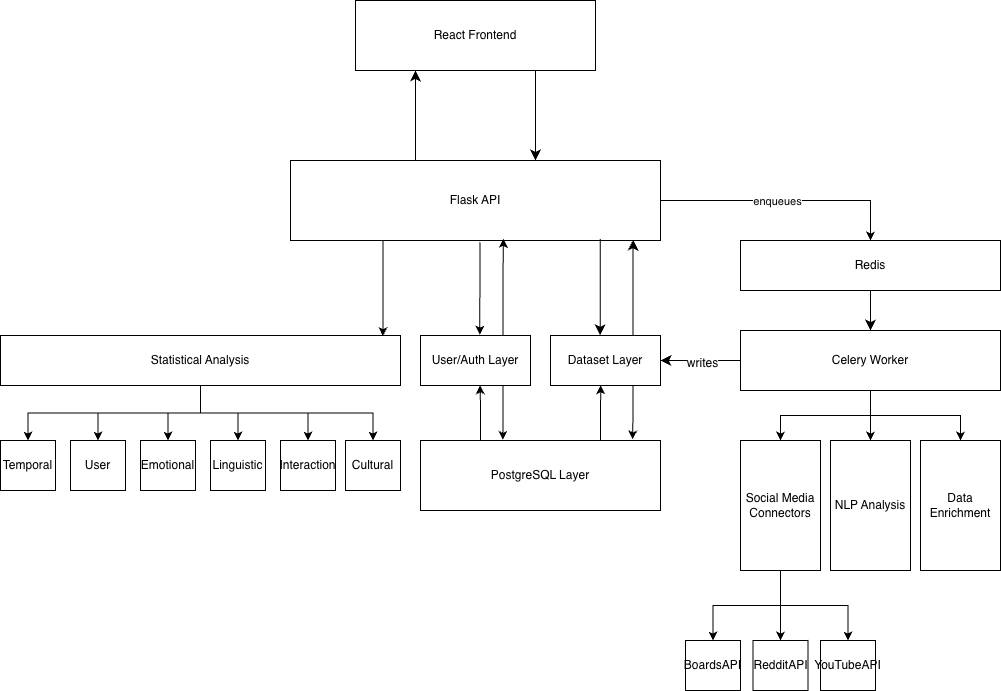
\includegraphics[width=1.0\textwidth]{img/architecture.png}
    \caption{System Architecture Diagram}
    \label{fig:architecture}
\end{figure}

\begin{figure}[h]
    \centering
    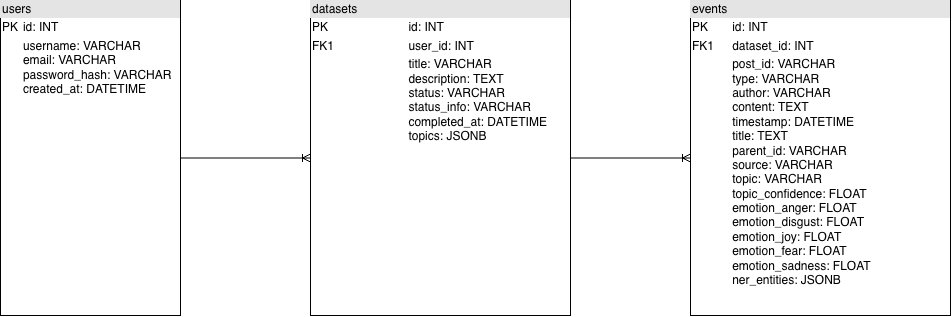
\includegraphics[width=1.0\textwidth]{img/schema.png}
    \caption{System Schema}
    \label{fig:schema}
\end{figure}

\subsection{Client-Server Architecture}
The system will follow a client-server architecture, with a Flask-based backend API and a React-based frontend interface. The backend will handle data processing, NLP analysis, and database interactions, while the frontend will provide an interactive user interface for data exploration and visualization.

The reasoning behind this architecture is that it allows the analytics to be aggregated and computed on the server side using Pandas which is much faster than doing it on the client frontend. The frontend will focus on rendering and visualising the data.

\subsubsection{API Design}
The Flask backend will expose a RESTful API with endpoints for dataset management, authentication and user management, and analytical queries. Flask will call on backend components for data parsing, normalisation, NLP processing and database interfacing. 

Flask was chosen for its simplicity, familiarity and speed of development. It also has many extensions that can be used for authentication (Flask-Bcrypt, Flask-Login).

The API is separated into three separate groups, \textbf{authentication}, \textbf{dataset management} and \textbf{analysis}. 

\subsubsection{React Frontend}
React was chosen for the frontend due to its massive library of pre-built components with efficient rendering capabilities and ability to display many different types of data. The frontend will be structured around a tabbed interface, with each tab corresponding to a different analytical endpoint (e.g., temporal analysis, linguistic analysis, emotional analysis). Each tab will fetch data from the backend API and render it using appropriate visualisation libraries (react-wordcloud for word clouds, react-chartjs-2 for charts, etc). The frontend will also include controls for filtering the dataset based on keywords, date ranges, and data sources.

\subsection{Data Pipeline}
As this project is focused on the collection and analysis of online community data, the primary component that must be well-designed is the data pipeline, which encompasses the processes of data ingestion, normalisation, enrichment, storage, and retrieval for analysis.

A unified data model is used to represent all incoming data, regardless of its original source or structure. This ensures that the same pipeline works across YouTube, Reddit and boards.ie data, and can be easily extended to new sources in the future.

\subsubsection{Data Ingestion}
The system will support two methods of data ingestion:
\begin{itemize}
    \item \textbf{File Upload}: Users can upload datasets in a specified \texttt{.jsonl} format, which contains posts and nested comments.
    \item \textbf{Automated Fetching}: Users can trigger the system to automatically fetch data from supported social media platforms using specified keywords or filters.
\end{itemize}

Originally, only file upload was supported, but the goal of the platform is to aid researchers with ethnograpic analysis, and many researchers will not have the technical expertise to fetch data from social media APIs or scrape websites. Therefore, the system was designed to support automated fetching of data from social media platforms, which allows users to easily obtain datasets without needing to manually collect and format data themselves.

In addition to social media posts, the system will allow users to upload a list of topics that they want to track in the dataset. This allows the system to generate custom topic analysis based on user-defined topics, which can be more relevant and insightful for specific research questions. For example, a researcher studying discussions around local politics in Cork might upload a list of political parties, politicians, and policy issues as topics to track.

Below is a snippet of what a custom topic list might look like in \texttt{.json} format:
\begin{Verbatim}[breaklines=true]
{
    "Public Transport": "buses, bus routes, bus eireann, public transport, late buses, bus delays, trains, commuting without a car, transport infrastructure in Cork",
    "Traffic": "traffic jams, congestion, rush hour, cars backed up, gridlock, driving in Cork, road delays",
    "Parking": "parking spaces, parking fines, clamping, pay parking, parking permits, finding parking in the city",
    "Cycling": "cycling in Cork, bike lanes, cyclists, cycle safety, bikes on roads, cycling infrastructure"
}
\end{Verbatim}

If a custom topic list is not provided by the user, the system will use a pre-defined generalised topic list that is designed to capture common themes across a wide range of online communities.

Each method of ingestion will format the raw data into a standardised structure, where each post will be represented as a "Post" object and each comment will be represented as a "Comment" object.

\subsubsection{Data Normalisation}
After a dataset is ingested, the system will normalise all posts and nested comments into a single unified "event" data model. This means that both posts and comments will be represented as the same type of object, with a common set of fields that capture the relevant information for analysis. The fields in this unified data model will include:
\begin{itemize}
    \item \texttt{id} - a unique identifier for the post or comment.
    \item \texttt{content} — the text content of the post or comment.
    \item \texttt{author} — the username of the content creator.
    \item \texttt{timestamp} — the date and time when the content was created
    \item \texttt{source} — the original platform from which the content was retrieved (e.g., Reddit, YouTube, Boards.ie).
    \item \texttt{type} — a field indicating whether the event is a "post" or a "comment".
    \item \texttt{parent\_id} — for comments, this field will reference the original id of the post it's commenting on.
    \item \texttt{reply\_to} - for comments, this field will reference the original id of the comment it's replying to. If the comment is a direct reply to a post, this field will be null.
\end{itemize}

The decision to normalise posts and comments into a single "event" data model allows the same analytical functions to be applied uniformly across all content, regardless of whether it was originally a post or a comment. This simplifies the data model and reduces the complexity of the analytical pipeline, since there is no need to maintain separate processing paths for posts and comments.

As part of this normalisation process, the dataset is also \textbf{flattened}, so rather than comments being nested within their parent posts as they are in the raw source data, all events are stored as a flat sequence of records. The relationships between posts and comments are preserved through the \texttt{parent\_id} and \texttt{reply\_to} fields. This allows for more efficient querying and analysis of the data, as well as simplifying the data model.

Overall, the data normalisation process unifies the structure of the dataset, and flattens the data into a format that makes analysis more efficient and easier.

\subsubsection{Data Enrichment}
After normalisation, the dataset is enriched with additional derived fields and NLP outputs. This includes:
\begin{itemize}
    \item \textbf{Datetime Derivations}: Fields such as day of week, hour of day, and week of year are derived from the raw timestamp and stored alongside the event, so they do not need to be recomputed on every query.
    \item \textbf{NLP Analysis}: The text content of each event is processed through NLP models to generate outputs such as emotion classification, topic classification, and named entity recognition.
\end{itemize}

NLP processing lets us perform much richer analysis of the dataset, as it provides additional layers of information beyond just the raw text content. After enrichment, the dataset is ready to be stored in the database and made available for analysis through the API endpoints.

\subsubsection{Data Storage}
The enriched dataset is stored in a PostgreSQL database, with a schema similar to the unified data model defined in the normalisation section, with additional fields for the derived data, NLP outputs, and user ownership. Each dataset is associated with a specific user account, and the system supports multiple datasets per user.

The \texttt{events} table in PostgreSQL contains the following fields:
\begin{itemize}
    \item \texttt{id}: a unique identifier for the event.
    \item \texttt{dataset\_id}: a foreign key referencing the dataset this event belongs to. If the dataset is deleted.
    \item \texttt{post\_id}: the original identifier of the post or comment as it appeared on the source platform.
    \item \texttt{type}: whether the event is a post or a comment.
    \item \texttt{author}: the username of the content creator.
    \item \texttt{content}: the text content of the event.
    \item \texttt{timestamp}: the Unix epoch time at which the content was created.
    \item \texttt{date}, \texttt{dt}, \texttt{hour}, \texttt{weekday}: datetime fields derived from the timestamp at ingestion time.
    \item \texttt{title}: the title of the post, if the event is a post. Null for comments.
    \item \texttt{parent\_id}: for comments, the identifier of the post it belongs to. Null for posts.
    \item \texttt{reply\_to}: for comments, the identifier of the comment it directly replies to. Null if the comment is a direct reply to a post.
    \item \texttt{source}: the platform from which the content was retrieved.
    \item \texttt{topic}, \texttt{topic\_confidence}: the topic assigned to the event by the NLP model, along with a confidence score.
    \item \texttt{ner\_entities}: a list of named entities identified in the content.
    \item \texttt{emotion\_anger}, \texttt{emotion\_disgust}, \texttt{emotion\_fear}, \texttt{emotion\_joy}, \texttt{emotion\_sadness}: emotion scores assigned to the event by the NLP model.
\end{itemize}

\subsubsection{Data Retrieval}
The stored dataset can then be retrieved through the Flask API endpoints for analysis. The API supports filtering by keywords and date ranges, as well as grouping and aggregation for various analytical outputs.

\subsection{Natural Language Processing}
The system will utilise pre-trained NLP models to perform emotion classification, topic classification, and named entity recognition on the text content of each event. These NLP outputs will be stored in the database alongside the raw content, allowing for efficient retrieval and analysis without needing to re-run the models on every query.

These will be implemented in a separate module that will be called during the data enrichment phase of the pipeline. The specific models used for each task will be selected based on their performance and suitability for the type of text data being analysed. This module will be called by the Celery worker during the data enrichment phase, and the outputs will be stored in the database for later retrieval.

\subsubsection{Emotional Classification}
Emotional Classification will be the bedrock of the ethnographic analysis, as it provides insight into the emotions of a community and how they relate to different topics and users. As mentioned in the feasibility analysis, the outputs of the emotion classification model should be interpreted as indicative patterns rather than definitive representations of user meaning, due to the limitations of NLP models.

Usage of simple VADER-based models is usually too-simplistic for the type of text data being analysed. Classifying posts into positive, negative and neutral categories is not nuanced enough to truly capture the emotional tone of a community. Therefore, the system will use a more complex model that can classify text into a wider range of emotions, which will allow for richer analysis of the emotions of the community.

\subsubsection{Topic Classification}
Topic classification will allow the system to classify specific posts into specific topics, which can be used to understand what a community is talking about, and in conjunction with emotional classification, how they feel about these topics as well. The system will support both a generalised topic classification model that can classify posts into a set of pre-defined general topics, as well as a custom topic classification model that can classify posts into user-defined topics based on a list of topics and descriptions provided by the user.

Initially, the system would have extract common themes and topics from the dataset by extracting common keywords and phrases, and then use these to generate a topic list. However, this approach was noisy and topics were often singular random words that did not have any overlap with each other, making topic classification less insightful. Therefore, specified or pre-defined topic lists will instead be used.

\subsubsection{Named Entity Recognition}
Named Entity Recognition allows the system to identify specific entities mentioned in the text, like people, places and organisations. In combination with emotional classification, we can see the general sentiment around specific places and people in a community, which can be very insightful for ethnographic analysis. For example, in a Cork-specific dataset, we might see that the city centre is often mentioned with negative emotions due to traffic and parking issues, while local parks are mentioned with positive emotions.

\subsection{Ethnographic Analysis}
The main goal of this project is to provide a tool that can assist researchers with ethnographic analysis of online communities. Therefore, ethnographic analysis will be a core component of the system.

Ethnographic analysis can be carried out from many different perspectives, such as the perspective of a single user or the community as a whole. The system is designed to support both of these perspectives, as well as the ability to zoom in and out between them. For example, a researcher might want to look at the overall emotional tone of a community, but then zoom in to see how a specific user contributes to that tone.

The system is designed to support multiple types of analysis, such as:
\begin{itemize}
    \item \textbf{Temporal Analysis}: looking at when a community is active and how that activity changes over time.
    \item \textbf{Linguistic Analysis}: looking at the words and phrases that are commonly used in a community, and how they relate to identity and culture.
    \item \textbf{Emotional Analysis}: looking at the emotional tone of a community, and how it varies across different topics or users.
    \item \textbf{User Analysis}: looking at the behaviour and activity of individual users, and how they contribute to the community.
    \item \textbf{Interaction Analysis}: looking at how users interact with each other, such as who replies to whom and how conversations develop.
    \item \textbf{Cultural Analysis}: looking at the cultural markers and identity signals that are present in a community, such as slang, memes, and recurring references.
\end{itemize}

Each of these types of analysis are available at different API endpoints for any given dataset, and the frontend is designed to allow users to easily switch between them and explore the data from different angles.

For each type of analysis that involves analysing the content of the posts themselves, they will be split into tokens and stop words will be stripped from them, which makes analysis easier.

\subsubsection{Temporal Analysis}
Temporal analysis allows researchers to understand what a community is talking about over time, and how the emotional tone of the community changes over time. For example, a researcher might want to see how discussions around a specific topic evolve over time, or how the emotional tone of a community changes in response to external events.

However a major limitation of the data captured for this system, whether it's the Cork dataset, or any automatically fetched dataset, it will only stretch at most a few weeks back in time. This is because the system is designed to fetch only the most recent posts and comments from social media platforms, which means that it will not capture historical data beyond a certain point. Therefore, while temporal analysis can still be carried out on the dataset, it will be limited to a relatively short timeframe.

In this system, temporal analysis will be limited to:
\begin{itemize}
    \item Event frequency per day.
    \item Weekday--hour heatmap data representing activity distribution.
\end{itemize}

\textbf{Average reply time per emotion} was considered as a potential temporal analysis metric, but was eventually excluded due to inconsistent and statistically insignificant results that yielded no meaningful analytical insight. 

\subsubsection{Linguistic Analysis}
Linguistic analysis allows researchers to understand the language and words used in a community. For example, a researcher might want to see what words are most commonly used in a community, or how the language used in a community relates to identity and culture.

In this system, linguistic analysis will include:
\begin{itemize}
    \item Word frequency statistics excluding standard and domain-specific stopwords.
    \item Common bi-grams and tri-grams from textual content.
    \item Lexical diversity metrics for the dataset.
\end{itemize}

The word frequencies and n-gram metrics were chosen because they can provide insights into the language and phrases used commonly in an online community, which is important for ethnographic analysis and understanding a community fully. Lexical diversity metrics such as the total number of unique tokens versus the total number of tokens can show if a specific culture often repeats phrases (like memes, slang etc.) or if they often have structured, serious discussion without repeating themeselves.

Outlining a list of stopwords is essential for linguistic analysis, as it filters out common words that wouldn't be useful for linguistic analysis. Stop Word lists can be provided by a Python library such as NLTK. 

In addition to standard stop words, the system also excludes link tokens such as "www", "http", and "https" from the word frequency analysis, as social media users will often include links in their posts and comments, and these tokens can become quite common and skew the word frequency results without adding meaningful insight.

\subsubsection{User Analysis}
User analysis allows researchers to understand the behaviour and activity of individual users within a community. For example, a researcher might want to see who the most active users are in a community, or how different users contribute to the overall emotional tone of the community.

In this system, user analysis will include:
\begin{itemize}
    \item Identification of top users based on activity.
    \item Per-user activity such as:
    \begin{itemize}
        \item Total number of events (posts and comments).
        \item Average emotion distribution across their events.
        \item Average topic distribution across their events.
        \item Comment-to-post ratio.
        \item Vocabulary information such as top words used and lexical diversity.
    \end{itemize}
\end{itemize}

Initially the user endpoint contained the interactional statistics as well, as a case could be made for the user analysis and interaction analysis being combined, however a distinction can be made between individual user analysis and user analysis on a larger, community-level scale focused on interactions. This allows the user endpoint to stay focused on singular user analysis while still using NLP outputs like emotions and topics.

Identifying top users allows us to see the most active and prolific posters in a community, which might often be site-specific bots that comment on every post or deleted users, which often show up as simply "[Deleted User]" and can aggregate together in statistics . An example might be a User Moderator bot on Reddit, seen below.

\begin{figure}[h]
    \centering
    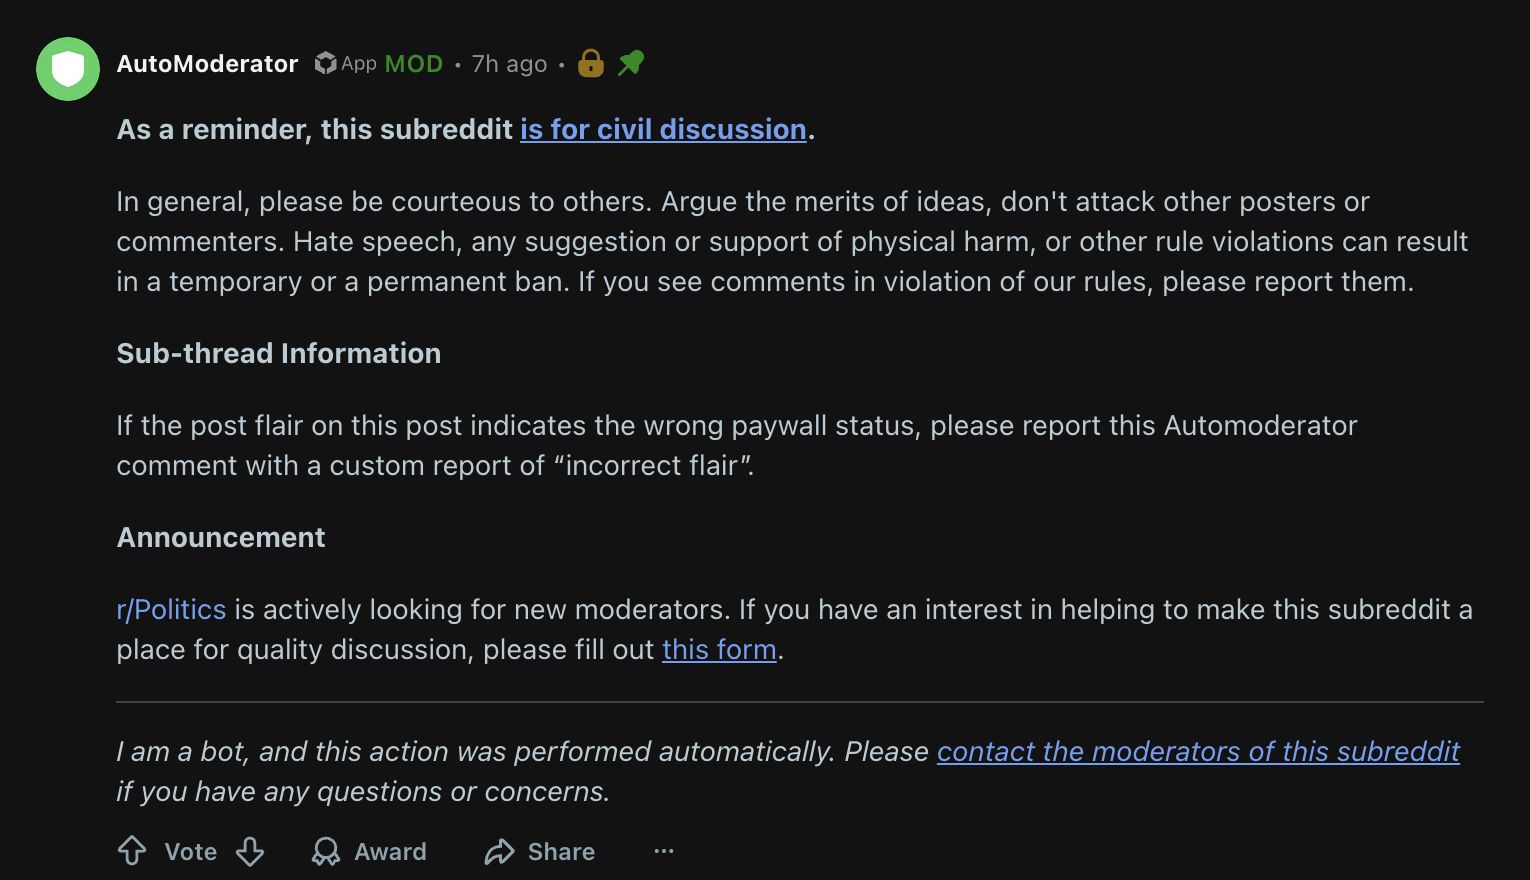
\includegraphics[width=0.75\textwidth]{img/reddit_bot.png}
    \caption{An AutoModerator Bot on r/politics}
    \label{fig:bot}
\end{figure}

While it's impossible to filter out all of these bots, deleted users can simply be filtered out using an exclusion list. 

\subsubsection{Interactional Analysis}
Instead of per-user analysis, interactional analysis looks at the interactions between users, such as who replies to who and who is contributing the most to the conversations. 

In this system, interactional analysis will include:
\begin{itemize}
    \item Top interaction pairs between users.
    \item An interaction graph based on user relationships.
    \item Conversation concentration metrics such as who is contributing the most to the conversations and how much of the conversation is dominated by a small number of users.
\end{itemize}

For simplicity, an interaction is defined as a reply from one user to another, which can be either a comment replying to a post or a comment replying to another comment. The system will not attempt to capture more complex interactions such as mentions or indirect references between users, as these would require more advanced NLP techniques.

\textbf{Average reply chain depth} was considered as a metric, however forum-based social media sites, such as boards.ie, do not have a way to reply to comments in the same way that Reddit does, therefore the concept of "reply chains" doesn't apply cleanly in the same way. One possible solution is to infer reply relationships from explicit user mentions embedded in content of the post, but this is not a reliable method.

\subsubsection{Emotional Analysis}
Emotional analysis allows researchers to understand the emotional tone of a community, and how it varies across different topics and users.

In this system, emotional analysis will include:
\begin{itemize}
    \item Average emotional by topic.
    \item Overall average emotional distribution across the dataset.
    \item Dominant emotion distributions for each event
    \item Average emotion by data source
\end{itemize}

It is emphasised that emotional analysis is inaccurate on an individual post level as the models cannot fully capture the nuance of human interaction and slang. Warnings will be presented to the user in the frontend that AI outputs can possible be misleading on an individual scale, and accuracy only increases with more posts. Even then it will not be perfect.

In an ideal world, the models are accurate enough to capture general emotions on a macro-scale.

\subsubsection{Cultural Analysis}
Cultural analysis allows researchers to understand the cultural markers and identity signals that are present in a community, such as slang, memes, and recurring references. While some of this is covered in the linguistic analysis, cultural analysis will focus more on the identity and stance-related markers that are present in the language of the community.

In this system, cultural analysis will include:
\begin{itemize}
    \item In-Group vs Out-Group phrasing 
    \item Average emotion for in-group vs out-group phrasing
    \item Stance Markers
    \item Average emotions per stance marker type
    \item Average emotions per entity
\end{itemize}

\subsection{Frontend Design}
The frontend is built with React and TypeScript, and the analysis sections are structured around a tabbed dashboard interface where each tab corresponds to a distinct analytical perspective: temporal, linguistic, emotional, user, and interaction analysis. This organisation mirrors the shape of the backend API and makes it straightforward for a researcher to navigate between different lenses on the same dataset without losing context.

React was chosen for its efficient rendering model and the breadth of its visualisation ecosystem


\subsection{Automatic Data Collection}
Originally, the system was designed to only support manual dataset uploads, where users would collect their own data from social media platforms and format it into the required \texttt{.jsonl} format. 

However, this approach is time consuming and since this system is designed to aid researchers rather than burden them, the system includes functionality to automatically fetch data from social media platforms. This allows users to easily obtain datasets without needing to manually collect and format data themselves, which is especially beneficial for researchers who may not have technical expertise in data collection.

The initial system will contain connectors for:
\begin{itemize}
    \item \textbf{Reddit} — using the official Reddit API to fetch posts and comments from specified subreddits or filtered by keywords.
    \item \textbf{YouTube} — using the YouTube Data API v3 to fetch video comments based on search queries.
    \item \textbf{Boards.ie} — using web scraping techniques to collect posts and comments from the Cork section of the Boards.ie forum.
\end{itemize}

\subsubsection{Connector Abstractions}
While the system is designed around a Cork-based dataset, it is intentionally source-agnostic, meaning that additional data sources for data ingestion could be added in the future without changes to the core analytical pipeline.

\textbf{Data Connectors} are components responsible for fetching and normalising data from specific sources. Each connector implements a standard interface for data retrieval.

Creating a base interface for what a connector should look like allows for the easy addition of new data sources in the future. For example, if a new social media platform becomes popular, a new connector can be implemented to fetch data from that platform without needing to modify the existing data pipeline or analytical modules.

The connector registry is designed so that any new connector implementing \texttt{BaseConnector} is automatically discovered and registered at runtime, without requiring changes to any existing code. This allows for a modular and extensible architecture where new data sources can be integrated with minimal effort.

\subsection{Asynchronous Processing}
The usage of NLP models for tasks such as sentiment analysis, topic classification, and entity recognition can be computationally intensive, especially for large datasets. In addition, fetching large datasets from sites like Reddit and YouTube takes a lot of time, due to the sequential nature of data fetching and severe rate limits on even authenticated Reddit accounts. To prevent the Flask API from blocking while these tasks are being processed, an asynchronous processing queue will be implemented using \textbf{Redis} and \textbf{Celery}.

\subsubsection{Dataset Enrichment}
A non-normalised dataset will be passed into Celery along with the dataset id and the user id of the dataset owner. At this point, the program is running separately to the main Flask thread. The program then calls on the \textbf{Normalisation \& Enrichment Module} to:
\begin{itemize}
    \item Flatten the dataset from posts with nested comments to unified event data model.
    \item Add derived timestamp columns to aid with temporal analysis
    \item Add topic, emotional and entity NLP analysis as columns
\end{itemize}

\subsubsection{Data Fetching}
If the user triggers a data auto-fetch from any given social media site, a task will be added to the Redis queue. Celery workers will then pop tasks off the Redis queue and process these tasks in the background, which ensures the API to remain responsive to user requests. The specific data connectors are called and the data fetching begins. Once the data has been fetched from all social media sites, NLP processing begins and we are at the same stage as before.

Asynchronous processing is especially important for automatic data-fetching, as particularly large datasets can take hours to fetch.


\subsection{Design Tradeoffs}
\subsubsection{Database vs On-Disk Storage}
Originally, the system was designed to store \texttt{json} datasets on disk and load them into memory for processing. This was simple and time-efficient for early development and testing. However, as the functionality of the system expanded, it become clear that a more persistent and scalable storage solution was needed.

Storing datasets in a database allows for more efficient querying, filtering, and updating of data without needing to reload entire datasets into memory. However the priamry benefit of using a database is support for \textbf{ multiple users and multiple datasets per user}. 

An additional benefit of using a database was that it allowed the NLP processing to be done once, with the NLP results stored alongside the original data in the database. This meant that the system could avoid redundant NLP processing on the same data, which was a significant performance improvement.

\texttt{PostgreSQL} was chosen as the database solution due to its robustness, support for complex queries, and compatibility with Python through \texttt{psycopg2}. PostgreSQL's support for JSONB fields allows for storage of unstructured NLP outputs, which alternatives like SQLite does not support.

\subsubsection{Unified Data Model vs Split Data Model}
The choice between a \textbf{Unified Data Model} and a \textbf{Split Data Model} led to many swaps in design for the API. 

\paragraph{The Case for a Unified Data Model}
\begin{itemize}
    \item \textbf{Simpler Schema}: One \texttt{events} table rather than split comments and posts tables
    \item \textbf{Simpler Pipeline}: The same pipeline works for both types
    \item \textbf{Differentiation Possible}: Through the \texttt{type} column, we can still differentiate between a post and a comment, though more awkwardly.
\end{itemize}

But it led to a simplification of some of the content, for example a post title is very different from the comment content. Reply chains must be reconstructed using the \texttt{reply\_to} and \texttt{parent\_id} fields and some fields, like \texttt{reply\_to} will be null depending on the data source. For example, boards.ie does not support nested replies.

\paragraph{The Case for a Split Data Model}
\begin{itemize}
    \item \textbf{Per-Type Analysis}: A post has different attributes to a comment, extending the analysis for post-specific metrics (like title sentiment, title-to-post length ratio) is easier later down the line.
    \item \textbf{Accurate Reply Relationship}: Reply relationships are naturally represented, comments have a foreign key to posts, no reconstruction needed.
\end{itemize}

However each analytical query would either need to be post or comment specific, or require a table merge later in the pipeline. For ethnographic analysis, the distinction between a post and a comment is minimal. From a research point of view a post and a comment are both just a user saying something at a point in time, and treating them uniformly reflects that.

The decision to \textbf{stick with a unified data model was made} since the downsides of a Unified Model could be mitigated through reconstruction of reply chains using specific fields, and being able to differentiate between a post and a comment using a type field. Largely, in ethnography, a post and a comment are both just a user saying something at a point in time, and even in cases where they might need to be treated differently (reply-chains, interactions graphs), that distinction can still be made.

\subsection{Deployment}
Docker Compose is used to containerise the entire application, including:
\begin{itemize}
    \item The Flask backend API
    \item The React frontend interface
    \item The PostgreSQL database
    \item The Redis server for task queuing
    \item Celery workers for asynchronous processing
\end{itemize}

During development, the source code for the backend and frontend will be mounted as volumes within the containers to allow for live code updates during development, which will speed up the process.

Enviornment variables, such as database credentials and social media API keys, will be managed through an \texttt{.env} file that is passed into the Docker containers through \texttt{docker-compose.yaml}.


\newpage
\section{Implementation}
In the previous chapter, the architecture of the web-based ethnography tool was
outlined. In this chapter, the details on how this was implemented will be
discussed.

\subsection{Overview}
In the initial stages, the project was a small Python script that would fetch data from Reddit and aggregate simple statistics such as number of posts and a number of comments. Some early features like search and subreddit specific searches were added through hard-coded variables. The Reddit Connector code was extracted into it's own \texttt{RedditConnector} module, though the connector abstraction had not yet been formalised.

As this was going to be a web-based tool, the Flask server was then setup. A rudimentary sentiment analysis endpoint was added as an initial test using the VADER Sentiment Python module. An endpoint to fetch from Reddit was added but temporarily scratched. Eventually more analysis endpoints were added, creating the many different analytical perspectives that are available in the final system, such as linguistic analysis and user analysis. 

At this stage, datasets were simply files stored on the machine and loaded into memory globally, which made early development and testing easier, but as the project progressed, the database was added to allow multiple datasets and users. While this was happening, further infrastructure was added to support multiple users, and to fix long-standing issues such as the blocking nature of NLP and data fetching, which was solved through the addition of Redis and Celery for asynchronous processing. Multiple user support was added through the addition of user accounts, with authentication and dataset ownership endpoints.

A very basic frontend was created with React, which was just a simple interface to call the API endpoints and display some basic summary stats such as number of posts, number of comments, and average sentiment. After the initial analysis endpoints were created and the API was fully functional, the frontend was expanded to include the full tabbed interface with visualisations for each analytical perspective.

\subsection{Project Tooling}
The project was developed using the following tools and libraries:
\begin{itemize}
    \item \textbf{Python 3.13} for the backend API and data processing.
    \item \textbf{Flask} for the web server and API development.
    \item \textbf{BeautifulSoup} and \textbf{Requests} for web scraping and HTTP requests.
    \item \textbf{google-api-python-client} for interacting with the YouTube Data API.
    \item \textbf{PostgreSQL} for the database.
    \item \textbf{Redis} and \textbf{Celery} for asynchronous task processing.
    \item \textbf{React} and \textbf{TypeScript} for the frontend interface.
    \item \textbf{Docker} and \textbf{Docker Compose} for containerisation and deployment.
    \item \textbf{Pandas} for data manipulation and analysis.
    \item \textbf{NLTK} for basic stop word lists and tokenisation.
    \item \textbf{Transformers} for NLP models used in emotion classification, topic classification, and named entity recognition.
    \item \textbf{react-chartjs-2} and \textbf{react-wordcloud} for data visualisation in the frontend.
\end{itemize}

The project was developed using Git for version control, with a branching strategy that included feature branches for new functionality and a main branch for stable code. Regular commits were made to document the development process and conventional commit messages were used to indicate the type of changes made. Occasionally, text bodies were included in commit messages to provide justification for design decisions or to explain changes that couldn't be easily understood from the diff alone.

\subsection{Social Media Connectors}
The first connectors implemented were the Reddit and Boards.ie connectors, as these were the original data sources for the Cork dataset. The YouTube connector was added later to improve diversity of data sources. In addition, the decision was made to only fetch new posts and fetch a fixed number of posts, rather than fetching the top posts of all time, which are usually full of memes and jokes that would skew the dataset and not be relevant for ethnographic analysis. In addition the temporal analysis would be skewed if we fetched top posts of all time, as the most popular posts are often from years ago, which would not be relevant for understanding the current state of the community.

\subsubsection{Data Transfer Objects}
Data Transfers Objects are simple classes that represent the data structure of a post or comment as it is retrieved from the source platform. They are used to encapsulate the raw data and provide a consistent interface for the rest of the system to interact with, regardless of the source platform.

These are later replaced by the unified "event" data model during the normalisation process, but they are a useful abstraction for the connectors to work with. Two DTOs are defined: \texttt{PostDTO} and \texttt{CommentDTO}, which represent the structure of a post and a comment respectively as they are retrieved from the source platform. The \texttt{PostDTO} will contain a list of \texttt{CommentDTO} objects.

\subsubsection{Reddit Connector}
The initial implementation of the Reddit connector was a simple class that simply used the \texttt{requests} library to fetch data directly from the Reddit API. The online Reddit API documentation was used as a reference for the implementation of the connector \cite{reddit_api}. It uses the \texttt{reddit.com/r/\{subreddit\}/new} endpoint to fetch the most recent posts from a specified subreddit, and the \texttt{reddit.com/r/\{subreddit\}/{post\_id}/comments} endpoint to fetch comments for each post.

It primary method implemented is of this signature:
\begin{Verbatim}[breaklines=true]
def get_new_posts_by_search(self, search: str, category: str, limit: int) -> list[Post]:
\end{Verbatim}

The \texttt{reddit.com/r/\{subreddit\}/new} has a default limit of 100 posts per request, therefore \textbf{pagination} was implemented to allow fetching of more than 100 posts, which is necessary for Reddit datasets of larger than 100 posts. The connector will keep fetching posts until it reaches the specified number of posts to fetch, or until there are no more posts available.

The "after" parameter is a post id and tells the API to fetch posts that come after that specific post id in the subreddit, which allows for pagination through the posts. The connector keeps track of the last post id fetched and uses it to fetch the next batch of posts until the desired number of posts is reached or there are no more posts available.

It became apparent that when unauthenticated, the Reddit API has severe rate limits that make fetching large datasets take hours, therefore the connector was updated to support authentication using Reddit API client credentials, which are provided through environment variables. This was done using the \texttt{requests\_oauthlib} library, which provides a convenient way to handle OAuth2 authentication with the Reddit API. With authentication, the rate limits are increased, allowing for faster data fetching.

\subsubsection{YouTube Connector}
The YouTube connector was the simplest out of the three initial connectors, as YouTube provides an official API that is well-documented compared to the Reddit API. The Python library \texttt{google-api-python-client} was used to interact with the YouTube Data API. It provides simple methods like \texttt{youtube.search().list()} to search for videos based on keywords, and \texttt{youtube.commentThreads().list()} to fetch comments for a specific video.

Like the Reddit Connector, it implements the \texttt{get\_new\_posts\_by\_search} method, which searches for videos based on a query and then fetches comments for those videos. As the Google API library handles comment fetching and pagination internally, the implementation was straightforward and did not require manual handling of pagination or rate limits.

\subsubsection{Boards.ie Connector}
The Boards.ie connector was the most complex connector to implement, as Boards.ie does not provide an official API for data retrieval, which meant web scraping techniques were utilised to fetch data from the site. The \texttt{requests} library was used to make HTTP requests to the Boards.ie website, and the \texttt{BeautifulSoup} library was used to parse the HTML content and extract the relevant data.

Inspect element was used to poke around the structure of the Boards.ie website and find the relevant HTML elements that contain the post and comment data. \texttt{BeautifulSoup} was then used to extract the correct data from the \texttt{.Message.userContent} tag and the \texttt{.PageTitle} tag, which contain the content and title of the posts. Each comment lived in an \texttt{ItemComment} class. Each of these were collected and iterated through to create the list of \texttt{PostDTO} and \texttt{CommentDTO} objects that represent the data retrieved from the site.

As not all comments on a thread are on one page, pagination was implemented by looking for the "Next" button on the page and following the link to the next page of comments until there are no more pages left. This allows for fetching of all comments for a given post, even if they span multiple pages.

A \texttt{ThreadPoolExecutor} was used to fetch posts in parallel, which improved the performance of the connector significantly, as fetching posts sequentially was very slow due to the need to fetch comments for each post, which often spanned multiple pages. Though there was diminishing returns after a certain number of threads, possibly due to site blocking or internet connection limits. Initially 20 threads were used, but this was later reduced to 10 threads to avoid potential issues with site blocking and to improve ethical considerations around web scraping.

\subsubsection{Connecter Plugin System}
The connector plugin system was implemented to allow for easy addition of new data sources in the future. This would require simply implemented a new connector class and dropping it into the connectors directory, without needing to modify any existing code. This was achieved through the use of Python's \texttt{importlib} library, which allows for dynamic importing of modules at runtime.

To achieve this, the base class \texttt{BaseConnector} was defined, which allows a standard interface for all connectors to implement. Each connector implements the \texttt{get\_new\_posts\_by\_search} method, which takes in a search query, a category (which is the subreddit for Reddit, or the category for Boards.ie), and a limit on the number of posts to fetch. The method returns a list of \texttt{PostDTO} objects that represent the data retrieved from the source platform.

In addition, some metadata is required for each connector, such as the source name, search support and category support, which are defined as class variables in each connector. This is required as some connectors may not support search or categories, for example YouTube does not support categories in the same sense that Reddit might.

\subsection{Database Configuration}
A PostgreSQL Docker container was set up to serve as the database for the system. This allows for persistent storage of datasets, as well as support for multiple users and multiple datasets per user. The implemented schema passed into the Docker container by mounting the \texttt{schema.sql} file as a volume, which allows for easy updates to the database schema during development. The database contains three main tables:
\begin{itemize}
    \item \textbf{users}: contains user information such as username, email and password hash.
    \item \textbf{datasets}: contains dataset information such as dataset name, description and owner (foreign key to users table).
    \item \textbf{events}: contains the main data for the posts and comments.
\end{itemize}

\subsubsection{Low-Level Connector}
A low-level \texttt{PostgreConnector} module was implemented to handle the raw SQL queries for interacting with the database. It connects to the Docker container using environment variables for the database credentials, which are passed into the container through the \texttt{docker-compose.yaml} file. The connector provides methods for executing queries with parameters and supports rollback in the case of errors.

 Two main methods of the connector are:
\begin{itemize}
    \item \texttt{def execute(self, query, params=None, fetch=False) -> list}
    \item \texttt{def execute\_batch(self, query, values) -> list}
\end{itemize}

This module provides a simple interface for executing SQL queries. It's used by higher level modules to interact with the database without needing to worry about the details of database connections and query execution.

\subsubsection{Dataset Manager}
The dataset manager is a higher-level module that provides an interface for managing datasets in the database. It uses the low-level \texttt{PostgreConnector} to execute SQL queries, but provides more specific methods for dataset management, such as creating a new dataset, fetching a dataset by id, and updating a dataset metadata. Dependency injection is used to pass an instance of the \texttt{PostgreConnector}.

The \texttt{DatasetManager} class is responsible for all database interactions relating to datasets, and draws a deliberate distinction between two categories of data:
\begin{itemize}
    \item \textbf{Dataset metadata} (the \texttt{datasets} table) refers to the metadata about a dataset like its name, owner, topic configuration, and processing status. Methods such as \texttt{save\_dataset\_info()}, \texttt{get\_dataset\_info()}, and \texttt{set\_dataset\_status()} operate on this layer.
    \item \textbf{Dataset content} (the \texttt{events} table) refers to the enriched event rows produced by the pipeline. \texttt{save\_dataset\_content()} performs a batch insert of the full enriched DataFrame, with NER entities serialised to JSONB via \texttt{psycopg2}'s \texttt{Json} wrapper, and emotion scores stored as flat numeric columns to allow direct SQL aggregation without requiring JSON parsing at query time.
\end{itemize}

\texttt{authorize\_user\_dataset()} enforces ownership by comparing the dataset's \texttt{user\_id} against the requesting user before any operation is performed, returning \texttt{False} rather than raising an exception so that the calling route handler can respond with an appropriate HTTP error.

NER output is stored as JSONB rather than in relational columns, as the number of extracted entities per post is arbitrary and varies between posts. Storing this into a fixed column structure would have been awkward and required a schema redesign.

This module is a simple interface to deal with datasets in the database, and abstracts away the details of SQL queries and database interactions from the rest of the application. It is used by the API endpoints to manage datasets and their content.

\subsubsection{Authentication Manager}
The authentication manager is another higher-level module that provides an interface for managing user authentication in the database. It also uses the low-level \texttt{PostgreConnector} to execute SQL queries, but provides more specific methods for authentication management, such as creating a new user, fetching a user by id, and authenticating a user. It handles password hashing using the \texttt{bcrypt} library, which provides a secure way to hash and verify passwords. Similar to the dataset manager, dependency injection is used to pass an instance of the \texttt{PostgreConnector}.

The most important authentication methods implemented are as follows:
\begin{itemize}
    \item \texttt{register\_user(username: str, email: str, password: str) -> None}: Registers a new user, hashes their password, checks for duplicate usernames or emails, and stores the user in the database.
    \item \texttt{authenticate\_user(username: str, password: str) -> None | dict}: Authenticates a user by verifying the provided password against the stored hash, returning user information if successful or \texttt{None} if authentication fails.
    \item \texttt{get\_user\_by\_id(user\_id: int) -> None | dict}: Fetches a user's information from the database based on their user ID, returning a dictionary of user details if found or \texttt{None} if no such user exists.
\end{itemize}

Defensive programming is used in the authentication manager to handle edge cases like duplicate usernames or emails, an example of this is in the \texttt{register\_user()} method, shown below:

\begin{Verbatim}[breaklines=true]
def register_user(self, username, email, password):
    hashed_password = self.bcrypt.generate_password_hash(password).decode("utf-8")

    if len(username) < 3:
        raise ValueError("Username must be longer than 3 characters")

    if not EMAIL_REGEX.match(email):
        raise ValueError("Please enter a valid email address")

    if self.get_user_by_email(email):
        raise ValueError("Email already registered")

    if self.get_user_by_username(username):
        raise ValueError("Username already taken")

    self._save_user(username, email, hashed_password)
\end{Verbatim}

This module is a simple interface that the higher level Flask API can call for easy management of user authentication and registration.

\subsection{Data Pipeline}
The data pipeline began with the data connectors mentioned in the previous section, which are responsible for fetching raw data from the source platforms. However they were not initially included as part of the data pipeline, as the initial system was designed to only support manual dataset uploads. The data connectors were used to fetch data for the Cork dataset, which was then uploaded automatically through the API. Once the automatic data fetching functionality was added, the connectors were integrated into the data pipeline.

\subsubsection{Data Enrichment}
The data enrichment process is responsible for taking the raw data retrieved from the connectors and transforming it into a format that is suitable for analysis. This involves several steps, including normalisation, NLP processing, and storage in the database.

Data Normalisation was intended to be a separate step in the data pipeline, but it was later combined with the enrichment processe as normalisation is a very small part of the process and can be done in a few lines of code, therefore it was combined with data enrichment. In normalisation, the list of \texttt{Post} objects retrieved from the connectors is flattened into a unified list of "events", which is a Pandas DataFrame that contains both posts and comments in a single table. The structure of the comments expansion method is as follows:
\begin{itemize}
    \item The method receives a DataFrame \texttt{df} where each row represents a post, and the \texttt{comments} column contains a list of comment dictionaries.
    \item The \texttt{comments} column is exploded using \texttt{pandas.DataFrame.explode()}, so that each comment occupies its own row, paired with the \texttt{id} of its parent post.
    \item Rows where the comment value is not a dictionary are filtered out, discarding any \texttt{None} or malformed entries that may have resulted from posts with no comments.
    \item \texttt{pd.json\_normalize()} is applied to the remaining comment dictionaries, flattening them into a structured DataFrame with one column per field.
    \item The original DataFrame is stripped of its \texttt{comments} column to form \texttt{posts\_df}, and a \texttt{type} column is added with the value \texttt{"post"}, along with a \texttt{parent\_id} column set to \texttt{None}, as posts have no parent.
    \item The comments DataFrame is similarly tagged with \texttt{type = "comment"}, and its \texttt{parent\_id} is populated from the \texttt{post\_id} field, establishing the relationship back to the originating post.
    \item Both DataFrames are concatenated using \texttt{pd.concat()}, and the now-redundant \texttt{post\_id} column is dropped, yielding a single unified events table containing both posts and comments with a consistent schema.
\end{itemize}

The \texttt{enrich()} method is the primary method for dataset enrichment in the module, and provides two main functionalities:
\begin{itemize}
    \item \textbf{Column Derivation}: This involves adding new columns to the dataset that are derived from existing data, such as timestamp parsing to extract date and time components.
    \item \textbf{NLP Analysis}: NLP analysis is performed on the dataset to add new columns that contains NLP outputs. The NLP performed includes emotion classification, topic classification, and named entity recognition.
\end{itemize}

Column derivation is a process of combining or altering existing columns to create new columns useful to analysis. The original dataset contains a timestamp column that might need to be parsed into a datetime format, and then new columns can be derived from this, such as the date, time, weekday, hour of the event, which is needed for temporal analysis like heatmaps. Datetime parsing on it's own is not usually intensive, but multiplied across thousands of posts and comments, it can add up, therefore it's calculated before analysis.

\subsubsection{Data Storage}
Once the dataset is enriched, it is ready for storage. Datasets are stored in a PostgreSQL database. The dataset manager is used to handle the storage of datasets in the database, and it provides a simple interface for saving the enriched dataset content. The enriched dataset is stored in the \texttt{events} table, with each row representing an event (either a post or a comment).

One issue arose using dependency injection for the dataset manager. Since from the data enrichment stage onwards, the data pipeline runs on a separate Celery worker process, therefore dependency injection of non-serialisable objects like \texttt{PostgresConnector} or \texttt{DatasetManager} does not work, as these objects cannot be passed through the Redis queue. To solve this, the \texttt{PostgresConnector} and \texttt{DatasetManager} are instantiated within the Celery worker process itself, rather than being passed in from the Flask API. While this introduces some tight coupling and possible synchronisation issues, these are not issues at this scale of project since both the Celery worker and database module use single-threaded connections to the database, but it's worth noting that this could be an issue if the project scaled up and had multiple Celery workers in parallel.

\subsection{NLP Module}
The NLP module is responsible for adding new columns to the dataset that contain the NLP outputs, three types of NLP analysis are performed: emotion classification, topic classification, and named entity recognition. It is instantiated once per dataset during the enrichment phase and runs on the provided Pandas DataFrame.

\subsubsection{Emotion Classification}
For emotional classification, initially a pre-trained VADER sentiment analysis model was used, which provides a very simple way to classify text into positive, negative, and neutral emotions. Though for ethnographic analysis, a more complex emotional model that can capture more nuance is needed, therefore the VADER model was later replaced with a fine-tuned transformer-based model that can classify text into a wider range of emotions. 

GoEMOTION \cite{demszky2020goemotions} was considered as a potential model for emotional classification, as it is extremely nuanced and can capture a wide range of emotions, however it had over 27 emotion classes, which was too many for the purposes of this project, as it would have been difficult to visualise and analyse such a large number of emotion classes. 

A middle ground was found with the "Emotion English DistilRoBERTa-base" model from HuggingFace \cite{hartmann2022emotionenglish}, which is a fine-tuned transformer-based model that can classify text into 6 emotion classes: anger, disgust, fear, joy, sadness, and surprise. This model provides a good balance between nuance and simplicity for the purposes of ethnographic analysis.

\subsection{Ethnographic Statistics}
This section will discuss the implementation of the various ethnographic statistics that are available through the API endpoints, such as temporal analysis, linguistic analysis, emotional analysis, user analysis, interactional analysis, and cultural analysis. Each of these are available through the API and visualised in the frontend. 




\subsection{Flask API}

\subsection{React Frontend}

\newpage
\section{Evaluation}

\newpage
\section{Conclusions}

\bibliography{references}

\end{document}
